\chapter{Farbe}
Was ist Farbe?
\begin{itemize}[labelindent=1cm]
  \item \textit{phsykalisch} Zusammensetzung des Lichts, das auf das Auge trifft.
  \item \textit{physiologisch} Wahrnehmung dieses Lichts im Auge und Interpretation
\end{itemize}


\section{Physikalische Grundlagen}
Licht besteht aus elektromagnetischer Strahlung verschiedener Wellenlänge.
\begin{description}[labelindent=1cm]
  \item[sichtbares Licht] Intervall von 380 nm (blau) bis 780 nm (rot)
  \item[infrarot] oberhalb von 780nm
  \item[ultraviolett] unterhalb von 380nm
\end{description}
Längeneinheit: 1nm = 10Å (Angström). Ein Atom hat etwa den Durchmesser von 1Å
\begin{figure}[!ht]
\centering
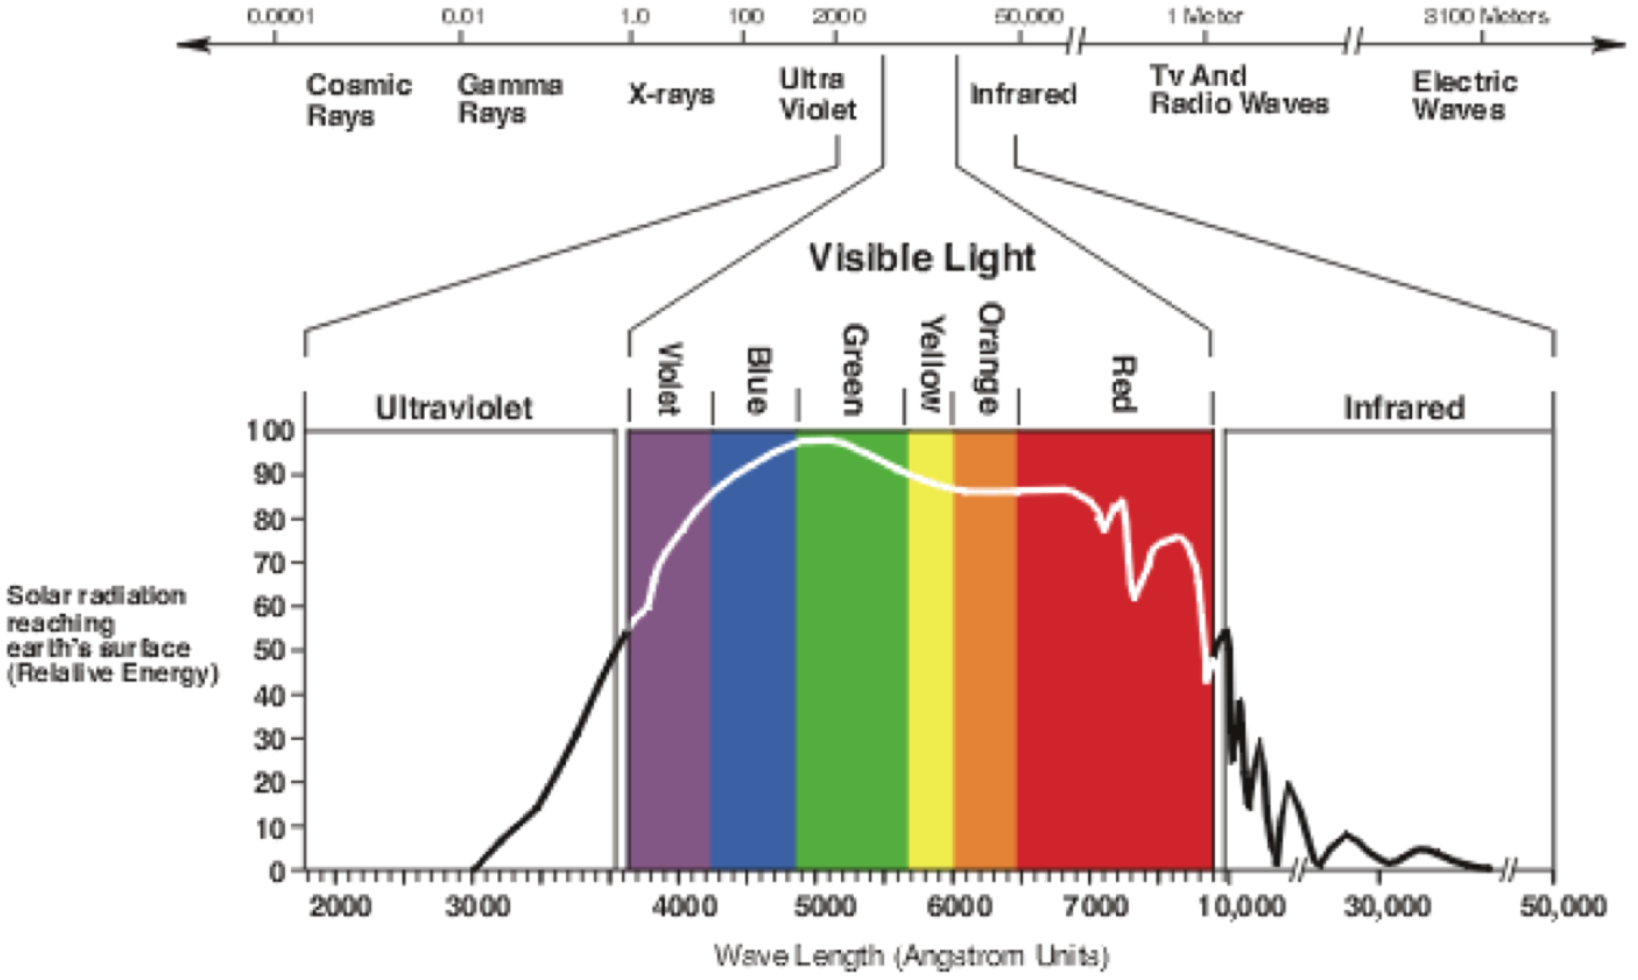
\includegraphics[width=0.7\linewidth]{fig/farbspectrum}
\caption{Farbspectrum}
\label{fig:farbspectrum}
\end{figure}

\subsection{Begriffe}
\begin{description}[labelindent=1cm]
  \item[Spektralfarben] haben genau eine Frequenz. Auch Spektralfarben haben Komplementärfarben.
  \item[Natürliches Licht] ist ein Mix aus Frequenzen.
  \item[Spektrum] ist die Verteilung der Frequenzen. Keine Frequenz sieht man Schwarz und wenn alle Frequenzen beteiligt, sieht man weiss. Wenn nur ein Teil der Frequenzen gibts eine Farbe.
  \item[Spektralverteilung] Dadurch können verschiedene Lichtquellen charakterisiert/unterschieden werden. Diese gibt an wie viel Energie in jeder Wellenlänge abgestrahlt wird. Es gibt verschiedene Spektralverteilungen, die als \textit{weiss} wahrgenommen werden.
  \item[Farbe einer Fläche] Licht fällt von einer Lichtquelle auf ein Objekt und wird von diesem zum Auge (oder zur Kamera) reflektiert.
  \item[Weitere Begriffe in der physikalischen Betrachtung] Lichtstärke, Lichtstromdichte, Leuchtdichte, Spezifische Lichtausstrahlung
\end{description}

\section{Farbwahrnehmung}
Wir nehmen Farben anders wahr als sie z.B. durch ihre physikalischen Eigenschaften definiert sind.\\
\textbf{Tristimulustheorie:} Auf der Netzhaut befinden sich 3 Arten von Zellen (Zäpfchen) , die auf Licht reagieren. Ihre höchste Empfindlichkeit liegt bei \textbf{rot, grün und blau}. Stäbchen und Zäpfchen bestimmen Auflösungsvermögen und Farbempfindlichkeit des Auges.
\begin{description}[labelindent=1cm]
  \item[Stäbchen $(75-150 \times 10^6)$] ermöglichen das Sehen bei niedriger Intensität. Nur Schwarz/Weiss-Sehen.
  
  \item[Zäpfchen $(6-7 \times 10^6)$] sind Fotorezeptoren für Licht höherer Intensität und für Farben. Fotopigmente sensibilisieren für rot (64\%), grün (32\%) und blau (4\%). Lange, mittlere und kurze Zäpfchen für lange (rot), mittlere (grün) und kurze Wellenlängen (blau). Die Zäpfchen sprechen jedoch auf einen ganzen Bereich von Wellenlängen an, nicht nur genau auf die Wellenlängen von rot, grün und blau. Neutraler werden sie daher auch als S, M und L bezeichnet.
\end{description}

  
\subsection{Wie sehen wir Farben}
\begin{itemize}
    \item Zäpfchen wirken wie ein Filter
    \item Farbe wird durch die Stärke der Antwort jeder Zäpfchensorte bestimmt: 3 Werte
    \item Damit kann nicht jede Spektraldichte repräsentiert werden
    \item Farben mit unterschiedlichen Spektren können also gleich aussehen: metamere Farben
\end{itemize}
\noindent
\textbf{WICHTIG:}\\Es ist also NICHT möglich jede Farbe mit rot, grün und blau zu mischen. Jedoch ein sehr grosser Anteil.
Das Tristimulustheorie-Experiment zeigte, dass die Kurven der Wellenlängen auch negativ sein können. D.h. man müsste Farben auch subtrahieren - was nicht geht. Beim Tristimulus hatten die Versuchspersonen drei Regler um die Farben Rot, Grün und Blau zu mischen. Der Versuchsleiter hatte einen Regler um durch sämtliche Spektralfarben zu gehen. Der Versuchsleiter stellte also eine Farbe ein und die Probanden mussten mit ihren drei Reglern versuchen, diese Farbe zu erreichen.

\clearpage
\section{Farbsysteme}
\subsection{Normfarbtafel}
Der Schnitt des 3D Farbraums mit der Ebene die durch (1,0,0), (0,1,0) und (0,0,1) geht ergibt die Normfarbtafel von CIE. Sie enthält alle Farbtöne. 
\begin{figure}[!ht]
\centering
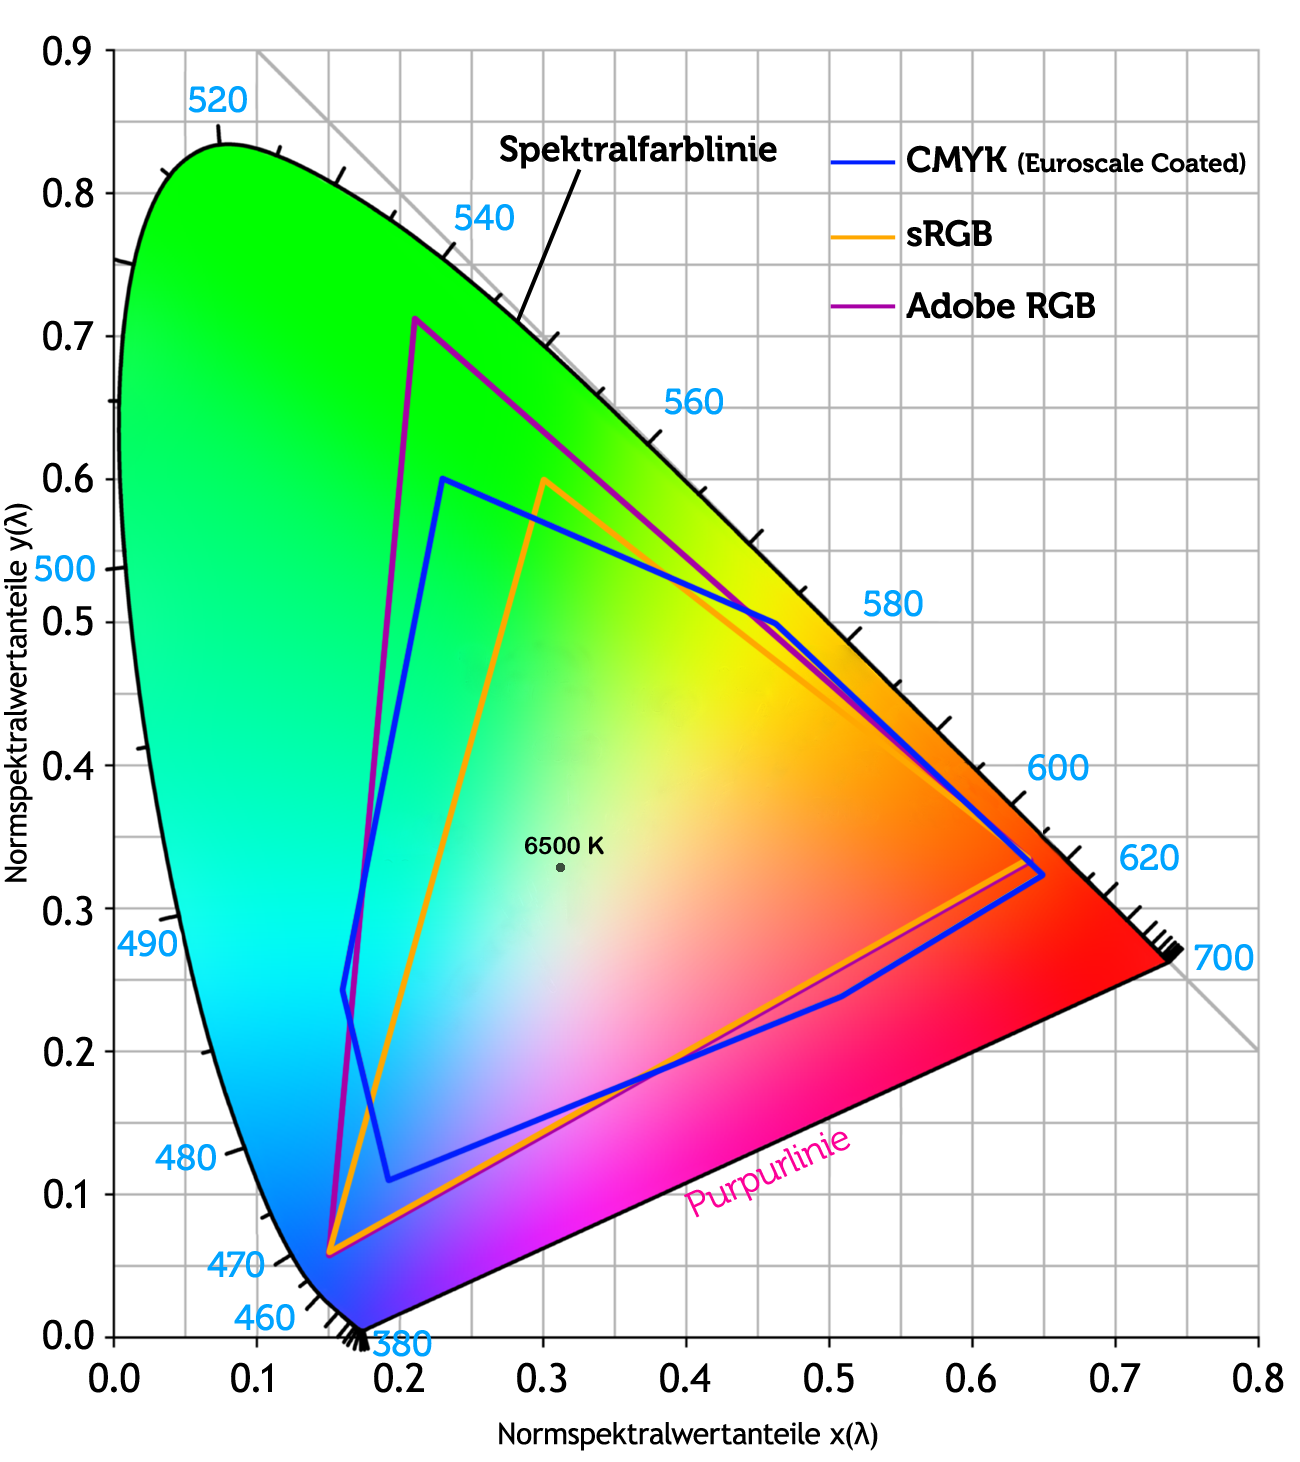
\includegraphics[width=0.4\linewidth]{fig/normfarbtafel}
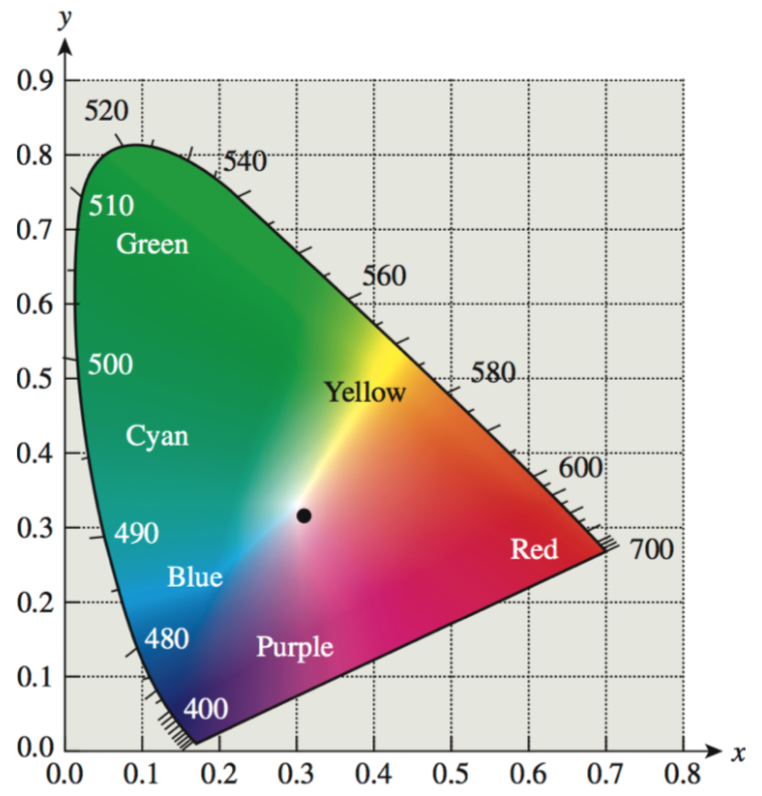
\includegraphics[width=0.4\linewidth]{fig/normfarbtafel2}
\caption{Normfarbtafel}
\label{fig:normfarbtafel}
\end{figure}

\subsubsection{Wichtige Eigenschaften}
\begin{itemize}[leftmargin=1cm]
    \item Sie enthält alle sichtbaren Farben in vollen Intensität
    \item Spektralfarben befinden sich am Rand (siehe Spektralfarbenlinie in Abb. \ref{fig:normfarbtafel} links)
    \item Der gerade Teil der Umrandung heisst \textit{Purpurlinie}
    \item \textbf{Mischen von Farben} Sind 2 Farben F1 und F2 auf der Tafel gegeben, so lassen sich mit ihnen alle Farben auf der Verbindungslinie zwischen F1 und F2 erzeugen.
    \item Dominante Wellenlänge kriegt man indem man die Farbe im Diagramm mit einem Punkt markiert. Dann zieht man vom Weiss eine Linie durch den Punkt bis an den Rand. Der Punkt am Rand ist dann die dominante Wellenlänge.
    \item Farben im unteren Teil des Diagramms besitzen keine dominante Wellenlänge und werden daher nicht spektral genannt.
    \item \textbf{Komplementärfarben} Farben die sich zu weiss addieren heissen Komplementärfarben. Das heisst, die Verbindungslinie zwischen zwei Komplementärfarben muss durch Weiss gehen.
\end{itemize}
\subsubsection{Farben am Monitor}
Ein bestimmter Monitor verwendet drei Farben (rot, grün, blau). Es können alle Farben in diesem Dreieck dargestellt werden (siehe Abb. \ref{fig:normfarbtafel} links) aber nicht alle der CIE Farbtafel. 


\subsection{Übersicht Farbsysteme}
Die meisten Farbsystem sind drei-dimensional und Stellen eine Farbe also durch 3 Komponenten dar.\\
Es gibt Hardware orientiere Farbsysteme:
\begin{itemize}[leftmargin=1cm]
    \item RGB für Bildschirme
    \item CMY(K) für die Drucktechnik
    \item YIQ (NTSC, Fernsehen USA/Japan)
    \item YUV, YCrCb: Video/TV-Farbsysteme (PAL, NTSC, SECAM)
\end{itemize}
\noindent
oder intuitive Farbsysteme wie
\begin{itemize}[leftmargin=1cm]
    \item HSV, HSI
    \item Munsell
    \item CIELab
\end{itemize}




\subsection{RGB} 
Ist ein additives Farbsystem. Eine Farbe wird durch 3 Grundfarben rot (R), grün (G) und blau (B) dargestellt. \\
C = (R, G, B)\\
Wertebereich für RGB ist das Intervall [0\dots1]. Dies kann allerdings auf 8bit (1 Byte) (0\dots255), 12bit oder 16bit abgebildet werden. Damit sind 16 Mio. Farben möglich.
\begin{figure}[!ht]
\centering
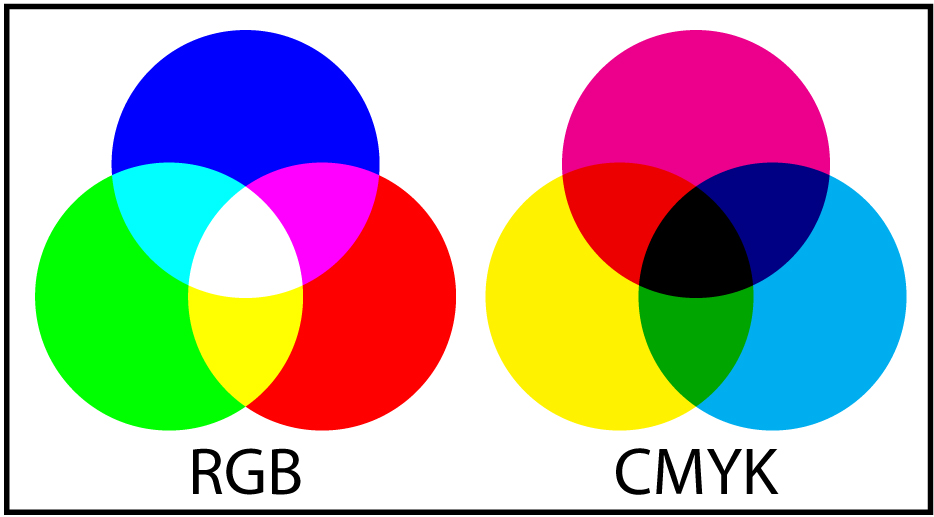
\includegraphics[width=0.7\linewidth]{fig/RGBvCMYK}
\caption{RGB (additives Farbsystem) vs. CMYK (subtraktives Farbssystem)}
\label{fig:rgbundcmyk}
\end{figure}
\subsubsection{Additive Mischung}
Bei der additiven Mischung von Farben empfängt das Auge die einzelnen Farben, der Farbeindruck entsteht durch die Addition der Spektren. Beispiel für additive Farbmischung:
\begin{itemize}[leftmargin=1cm]
    \item Monitore, Fernseher
    \item Scheinwerfer, Spotlights
    \item Kunst: Pointilismus
\end{itemize}


\subsection{CMYK} 
Wird beim Drucken eine Farbe auf eine Oberfläche aufgetragen, so absorbiert sie ein Teil des Lichtes. Werden mehrere Farbe aufgetragen, so wird nur derjenige Teil des Lichtes reflektiert, der von keiner Farbe absorbiert wurde. Farben addieren sich also nicht, sondern werden vom Licht subtrahiert, man nennt das auch subtraktive Farbmischung.\\
CMY ist ein Farbsystem für die subtraktive Farbmischung, es besteht aus den Komplementärfarben von RGB : C = cyan, M = magenta und Y = yellow. Die nachfolgende Auflistung zeigt welche Farben absorbiert bzw. reflektiert werden. Möchte man z.B. dass Grün reflektiert werden müssen yellow und cyan gemischt werden (absorbieren Blau und Rot).

\begin{tabbing}
	\hspace{4cm}\=\hspace{4cm}\=\kill
	Tintenfarbe \> absorbiert \> reflektiert \\
	\> \> \\
	Cyan \> Rot \> Grün und Blau \\
	Magenta \> Grün \> Blau und Rot \\
	Yellow \> Blau \> Rot und Grün \\
	Schwarz \> Alles \> Nichts 
\end{tabbing} 

Der Zusammenhang zwischen RGB und CMY ist also:

\begin{gather*}
\begin{pmatrix} C \\ M \\ Y \end{pmatrix} = 
\begin{pmatrix} 1 \\ 1 \\ 1 \end{pmatrix} -
\begin{pmatrix} R \\ G \\ B \end{pmatrix}
\end{gather*}
\begin{gather*}
C = B + G = W - R \\
M = R + B = W - G \\
Y = G + R = W - B \\
\end{gather*}

\noindent
Schwarz könnte zwar mittels C, M, Y gemischt werden, doch das Ergebnis ist schlecht (und auch zu teuer). Häufig wird deshalb noch Schwarz als vierte Farbe verwendet. Dieses System heisst CMYK (von blac\textbf{K}) und berechnet sich als:
\begin{gather*}
K = min(C, M, Y )\\
C = C - K \\
M = M - K \\
Y = Y - K \\
\end{gather*}

\subsection{HSV} 
HSV ist ein benutzerorientiertes Farbsystem, das sich nach der intuitiven Definition einer Farbe mittles Farbton, Sättigung und Helligkeit richtet:
\begin{center}
\begin{tabular}{ | l | l | p{7cm} | p{6cm} |}
\hline
H & Hue        & Farbton, spektraler Teil der Farbe; bestimmt ob Farbe rot, gelb, grün, etc & in Grad von 0 bis 360  (R=0, G=120, B=240)                              \\ \hline
S & Saturation & Sättigung, bestimmt die Reinheit der Farbe.                                & zwischen 0 (vollständig ungesättigt = Grauton) und 1 (gesättigte Farbe) \\ \hline
V & Value      & Helligkeit, Intensität.                                                    & zwischen 0 (schwarz) und 1 (volle Intensität)   \\     
\hline
\end{tabular}
\end{center}

\begin{figure}[!ht]
\centering
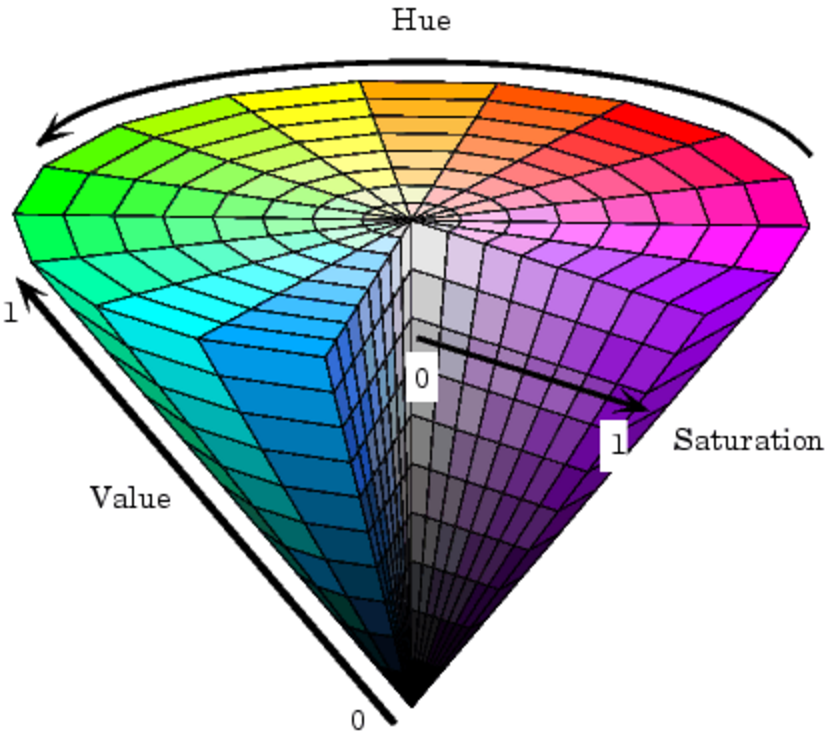
\includegraphics[width=0.4\linewidth]{fig/hsv1}
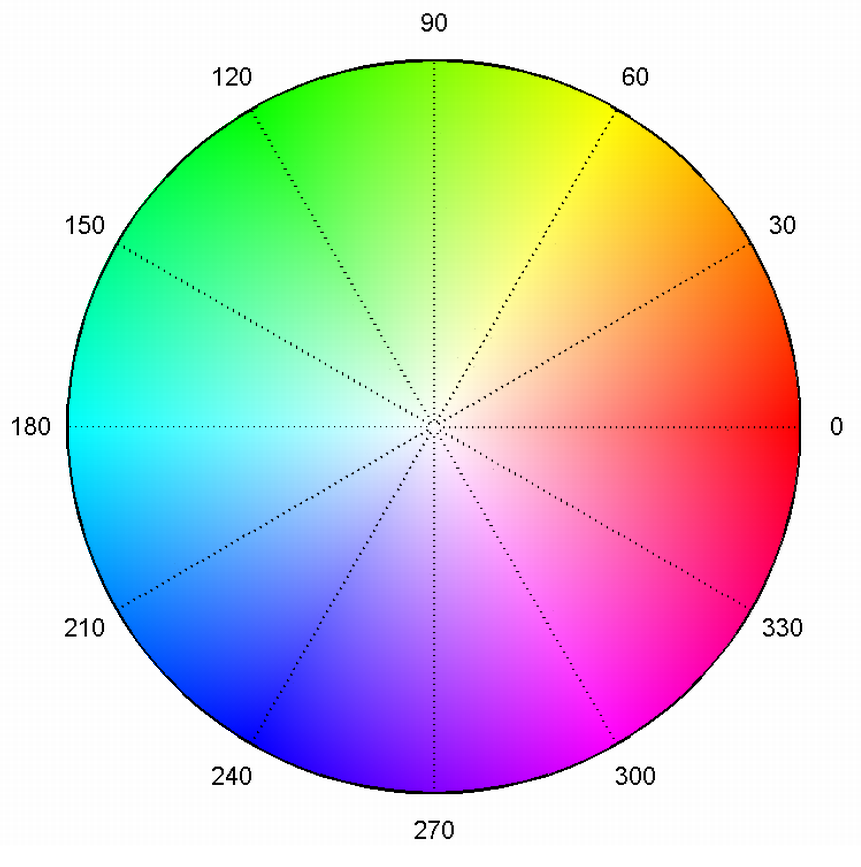
\includegraphics[width=0.4\linewidth]{fig/hsv2}
\caption{HSV}
\label{fig:hsv}
\end{figure}

\section{Halbtontechnik}
\subsection{Grauwerte}
Der Grauwert einer RGB-Farbe ist nicht der Mittelwert von R, G und B sondern:
\begin{gather*}
I = 0.299R + 0.587G + 0.114B
\end{gather*}
\begin{tabular}{|l|l|}
\hline
\rowcolor[HTML]{000000} 
{\color[HTML]{FFFFFF} \textbf{Farbe (in RGB)}} & {\color[HTML]{FFFFFF} \textbf{Grauwert (in RGB)}} \\ \hline
(255,0,0)                                      & (76,76,76)                                        \\ \hline
(0,128,0)                                      & (75,75,75)                                        \\ \hline
(200,200,200)                                  & (200,200,200)                                     \\ \hline
(255,200,128)                                  & (208,208,208)                                     \\ \hline
\end{tabular}


\subsection{Quantisierung}
Einfache aber nicht akzeptable Lösung. Die im ursprünglichen Bild verwendeten Farben, werden auf die Anzahl vorhandenen Farben quantisiert. 
\begin{figure}[!ht]
\centering
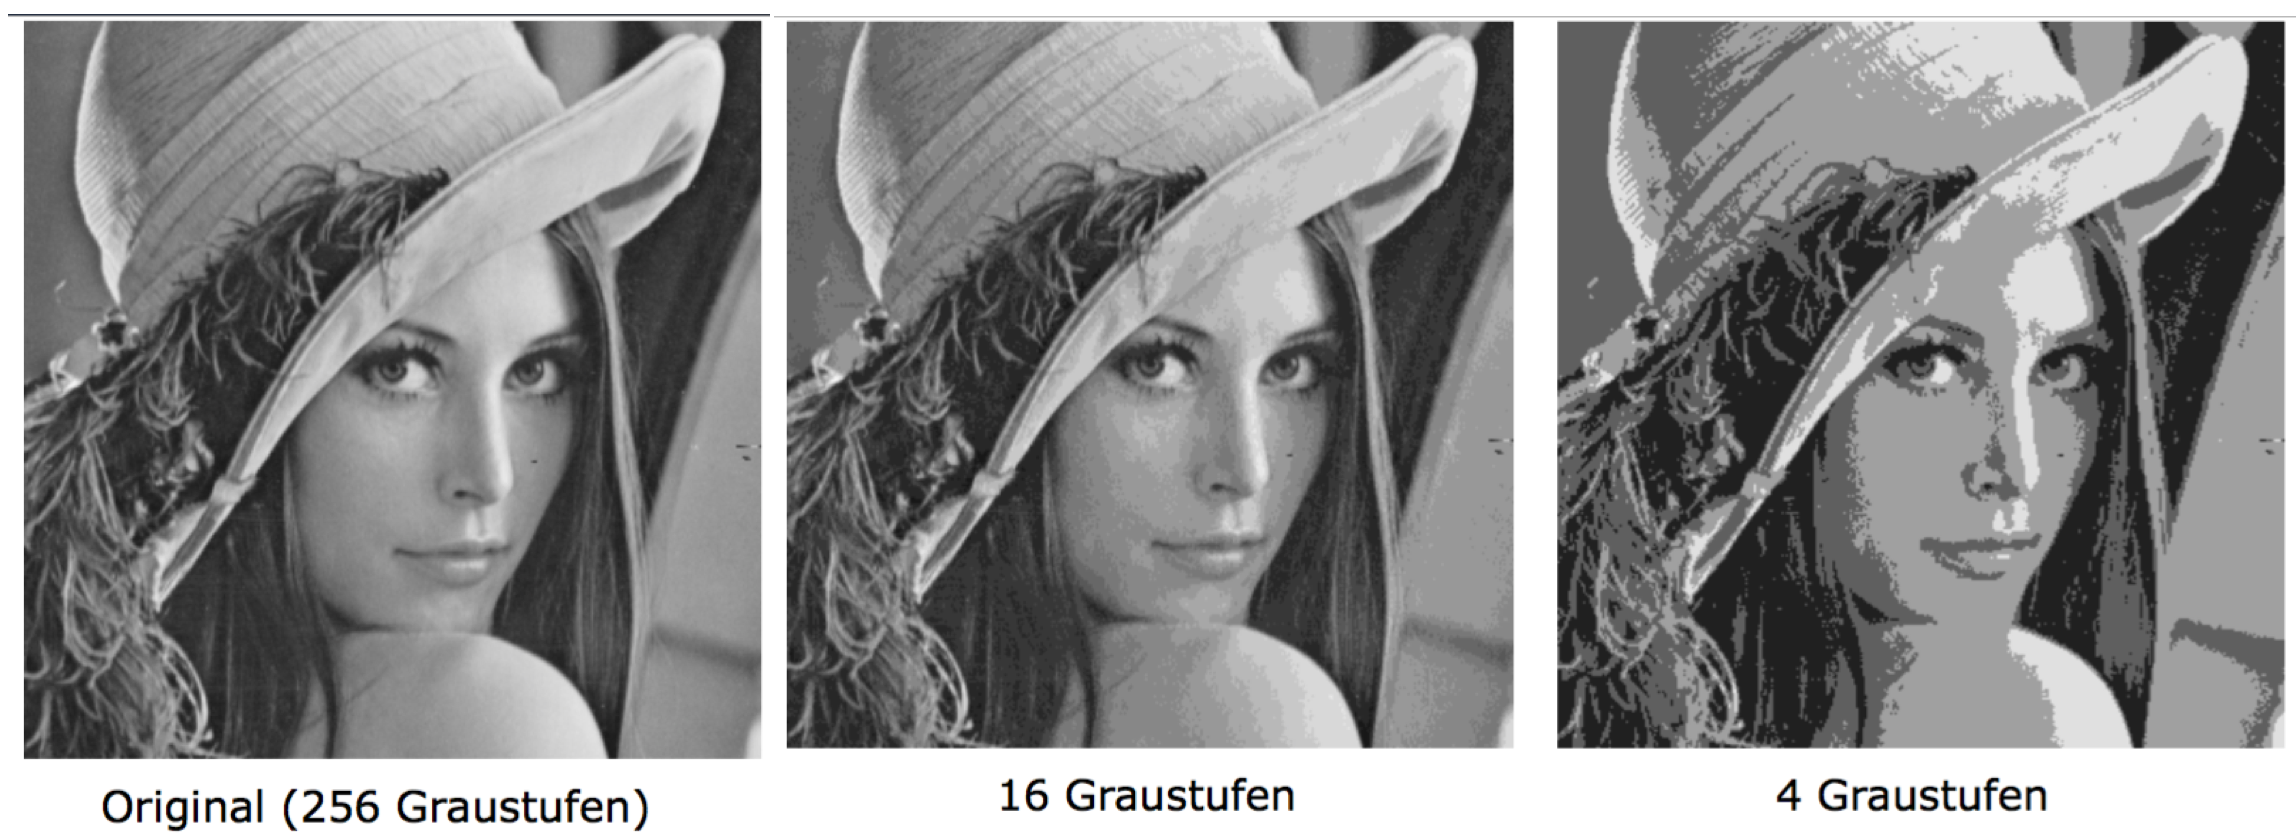
\includegraphics[width=0.8\linewidth]{fig/quantisierung}
\caption{Quantisierung}
\label{fig:Quantisierung}
\end{figure}
\subsubsection{Beispiel Konvertierung der Intensitätsstufen:}
Gegeben ist ein Bild mit Graustufen von 0-255. Es soll nun in 10 Stufen (3x3 Matrix) dargestellt werden. \(255 / 10 = 25.5 \)
\begin{figure}[!ht]
\centering
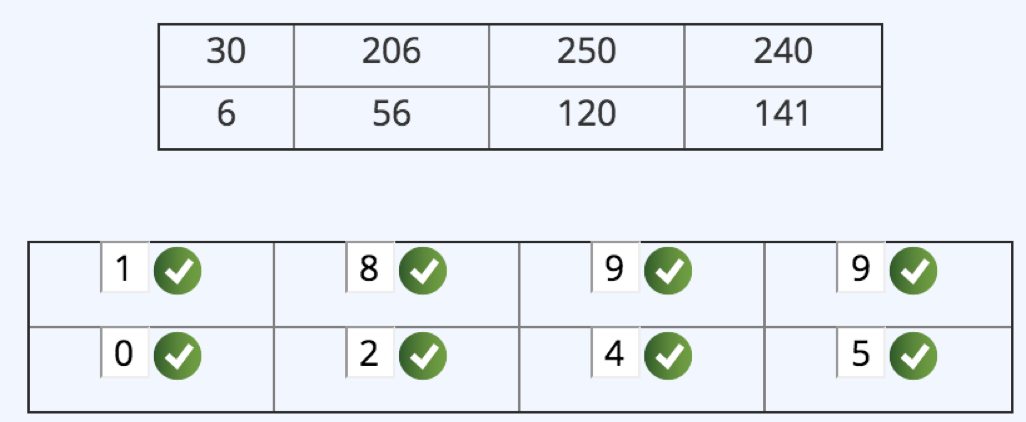
\includegraphics[width=0.5\linewidth]{fig/quantisierung_bsp}
\label{fig:quantisierung_bsp}
\end{figure}



\subsection{Dithering} 
Dithering wird verwendet um Farben auf einem Gerät zu simulieren, das weniger Farben darstellen kann. Jeder Pixel wird durch eine \(n \times n\)  Matrix ersetzt. Die Bildgrösse wird also vergrössert. Die Anzahl Intenistätsstufen ergibt sich durch  \((n \times n) + 1 \). Das heisst bei: 2x2 = 5 / 3x3 = 10 / 4x4 = 17
\begin{figure}[!ht]
\centering
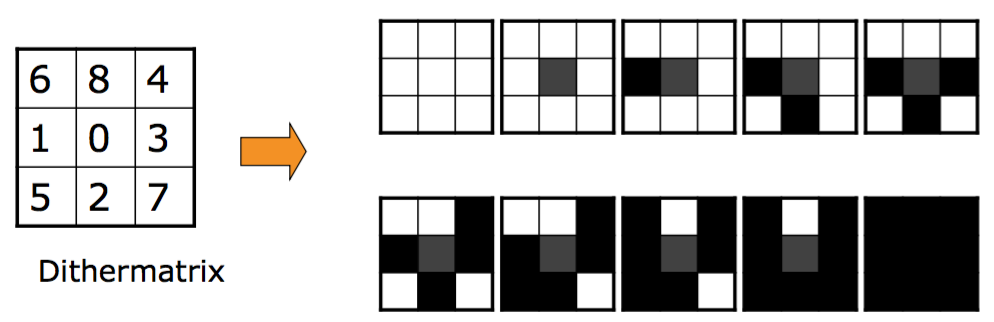
\includegraphics[width=0.7\linewidth]{fig/dithermatrix}
\label{fig:dithermatrix}
\end{figure}

\subsubsection{Wichtige Regeln für Dithering}
\begin{itemize}
    \item Strukturen sollten möglichst vermieden werden. Keine horizontale Streifen erzeugen (3 4 5; 1 0 2; 5 7 8)
    \item Es sollten möglichst Kreise approximiert werden.
    \item Einmal gefärbte Punkte sollen im nächsten Level gefärbt bleiben (ist bei der Verwendung von Dither-Matrizen automatisch der Fall)
\end{itemize}





\subsection{Dithering bei gleichbleibender Bildgrösse}
Hierzu gibt es folgende Methoden:
\subsubsection{Clustered dot dithering}
Berechnen des Mittelwert einer n x n Region und ersetzen der Region durch die Dithermatrix



\subsubsection{Dispersed dot dithering} 
Vergleich der einzelnen Pixel mit den Werten der Dithermatrix
Verwendet wird wieder eine n x n Matrix \(D_{ij}^{(n)}\). Für jeden Punkt wird
\begin{gather*}
i = x \mod n\\
j = y \mod n\\
\end{gather*}                                           
berechnet. Der Pixel wird gesetzt, falls seine Intensität grösser ist, als der Wert der Matrix.
\begin{gather*}
I(x,y) > D_{ij}^{(n)}   
\end{gather*}
Dieser Algorithmus wird Allgemein zur Reduktion der Graustufen/Farben verwendet, und nicht unbedingt nur zum Drucken von Bildern. Da ein Bildschirm individuelle Punkte viel besser darstellen kann als ein Drucker, muss die Matrix nicht allen oben beschriebenen Anforderungen genügen. Eine geeignete Matrix ist zum Beispiel die Bayes-Matrix
\begin{figure}[!ht]
\centering
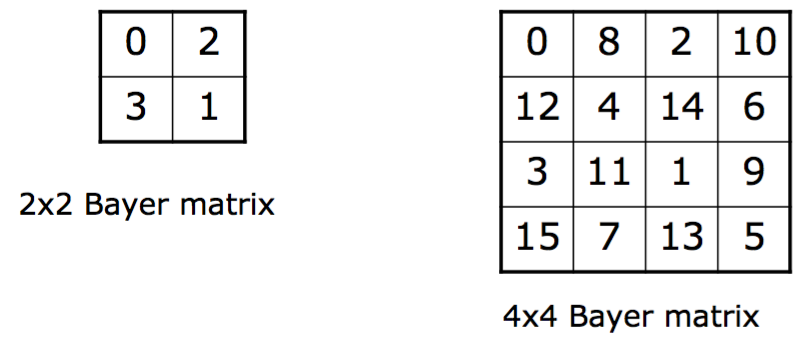
\includegraphics[width=0.5\linewidth]{fig/bayesmatrix}
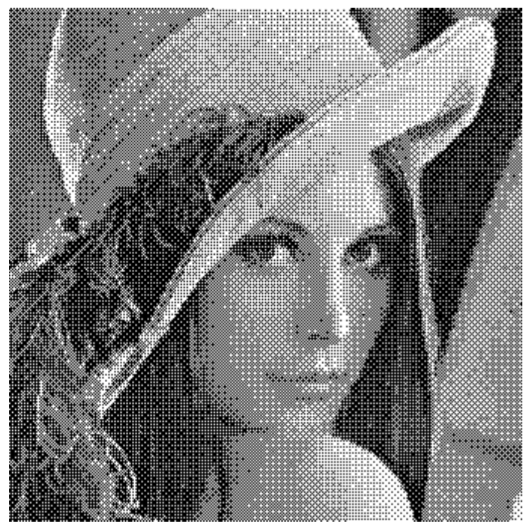
\includegraphics[width=0.3\linewidth]{fig/disperseddot}
\caption{Bayes Matrix (links) \& Dispersed Dot Dithering (rechts)}
\label{fig:bayesmatrix}
\end{figure}


\subsubsection{Dispersed Dot Dithering Quiz-Übung}
Ein Bild ist in den Grauwerten von 0-255 gegeben und soll auf einem Bildschirm dargestellt werden der nur 2 Farben zur Verfügung hat. Die Grösse sollte dabei nicht verändert werden. Geben Sie eine gesetzten Pixel mit 1, ungesetzten mit 0 an.

Man nehme die Ausgangstabelle:

\begin{table}[!ht]
	\centering
	\caption{Tabelle mit Pixelwerten von 0 - 255}
	\label{tbl:ausgangstabelle}
	\begin{tabular}{|l|l|l|l|}
		\hline
		30 & 200 & 250 & 240 \\ \hline
		6  & 56  & 120 & 141 \\ 
		\hline
	\end{tabular}
\end{table}

Wir haben hier jetzt eine 2x2 Dithermatrix:

\begin{displaymath}
D^2 = \begin{pmatrix}
0 & 3 \\
1 & 2
\end{pmatrix}
\end{displaymath}

Wir müssen nun die Werte von der Ausgangstabelle \(0-255\) auf den Wertebereich der Matrix \(0-3\) herunterskalieren. Wir berechnen daher den Faktor, mit dem wir jeden Pixelwert multiplizieren um ihn auf diesen Wertebereich hinunterzubringen.
\begin{displaymath}
k = \frac{W_{max}}{n*n+1}
\end{displaymath}

\begin{description}
	\item[\(\mathbf{W_{max}}\)] Maximalwert des Pixels (hier 255)
	\item[\(\mathbf{n}\)] Grösse (also Breite oder Höhe) der Matrix (hier 2)
	\item[\(\mathbf{k}\)] Resultierender Faktor
\end{description}
Der neue Wert eines Pixels berechnet sich dann einfach so:
\begin{displaymath}
W_{neu} = \lfloor W_{alt} * k \rfloor
\end{displaymath}
Wir erhalten dann folgende Zwischentabelle:

\begin{table}[!ht]
	\centering
	\caption{Tabelle für die Dithermatrix}
	\label{tbl:zwischentabelle}
	\begin{tabular}{|l|l|l|l|}
		\hline
		0 & 3 & 4 & 4 \\ \hline
		0  & 1  & 2 & 2 \\ 
		\hline
	\end{tabular}
\end{table}
Darüber legen wir nun einfach die Dithermatrix. Unsere Tabelle mit den Pixelwerten ist hier ja allerdings grösser als die Dithermatrix - dann legen wir sie einfach erneut hin, bis alles gefüllt ist. Mathematisch ausgedrückt setzen wir also hier eine 1 wenn folgender Ausdruck wahr ist:

\begin{displaymath}
	i = x \bmod n
\end{displaymath}
\begin{displaymath}
	j = y \bmod n
\end{displaymath}

\begin{description}
	\item[\(\mathbf{x}\)] Ausgangs X-Position Pixel 
	\item[\(\mathbf{y}\)] Ausgangs Y-Position Pixel
\end{description}

\begin{displaymath}
W_{x,y} > D_{i,j}
\end{displaymath}
Also wenn der Wert der Zwischentabelle grösser ist als der Wert in der Dithermatrix. Das Modulo Zeugs ist nur zum Mapping von der x Position des Pixels auf die Position innerhalb der Dither Matrix.

\begin{table}[!ht]
	\centering
	\caption{Resultat}
	\label{tbl:resultat_dither}
	\begin{tabular}{|l|l|l|l|}
		\hline
		0 & 0 & 1 & 1 \\ \hline
		0  & 0  & 1 & 0 \\ 
		\hline
	\end{tabular}
\end{table}


\subsubsection{Error Diffusion}
Anstatt Kreise verschiedener Grösse zu nehmen, können auch Punkte verschieden dicht angeordnet werden. (Frequenz-Verfahren). Die Idee dabei ist, dass der Fehler der durch das Setzen eines Pixels auf schwarz oder weiss gemacht wird, auf die umliegenden Pixel verteilt wird. Das Bild wird dabei sequentiell von oben nach unten und von links nach rechts durchlaufen. Der Fehler wird anhand der folgenden Gewichte auf die noch nicht besuchten Pixel verteilt:\\
\begin{figure}[!ht]
\centering
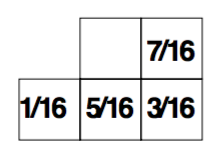
\includegraphics[width=0.2\linewidth]{fig/errordif2}
\end{figure}
\noindent
Der Algorithmus lautet als (für jeden Pixel (x;y)):\\
Error-Diffusion (nach Floyd und Steinberg):\\
\begin{figure}[!ht]
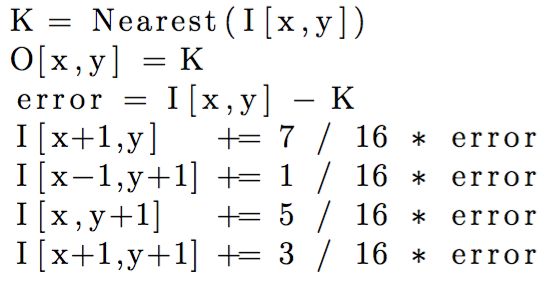
\includegraphics[width=0.4\linewidth]{fig/errordif1}
\end{figure}\\
\noindent
\textbf{Vorgehen bei Aufgabe} \\
\begin{enumerate}
  \item Zu verarbeitenden Pixel anschauen
  \item Bestimmen auf welchen Wert der Pixel gesetzt wird
  \item Fehler berechnen (Fehler = Differenz aus Neuer Wert und Ursprünglicher Wert)
  \item Den Rest gemäss Tabelle oben berechnen (Bsp. 7/16 * Fehler)
  \item Rest gemäss Formel auf umliegende Felder verteilen (Neuer Wert des Feldes = ursprünglichen Wert - Rest)
\end{enumerate}

\clearpage
\section{Cheat-Sheet}
\subsection{Farbumrechnung}
\begin{figure}[!ht]
	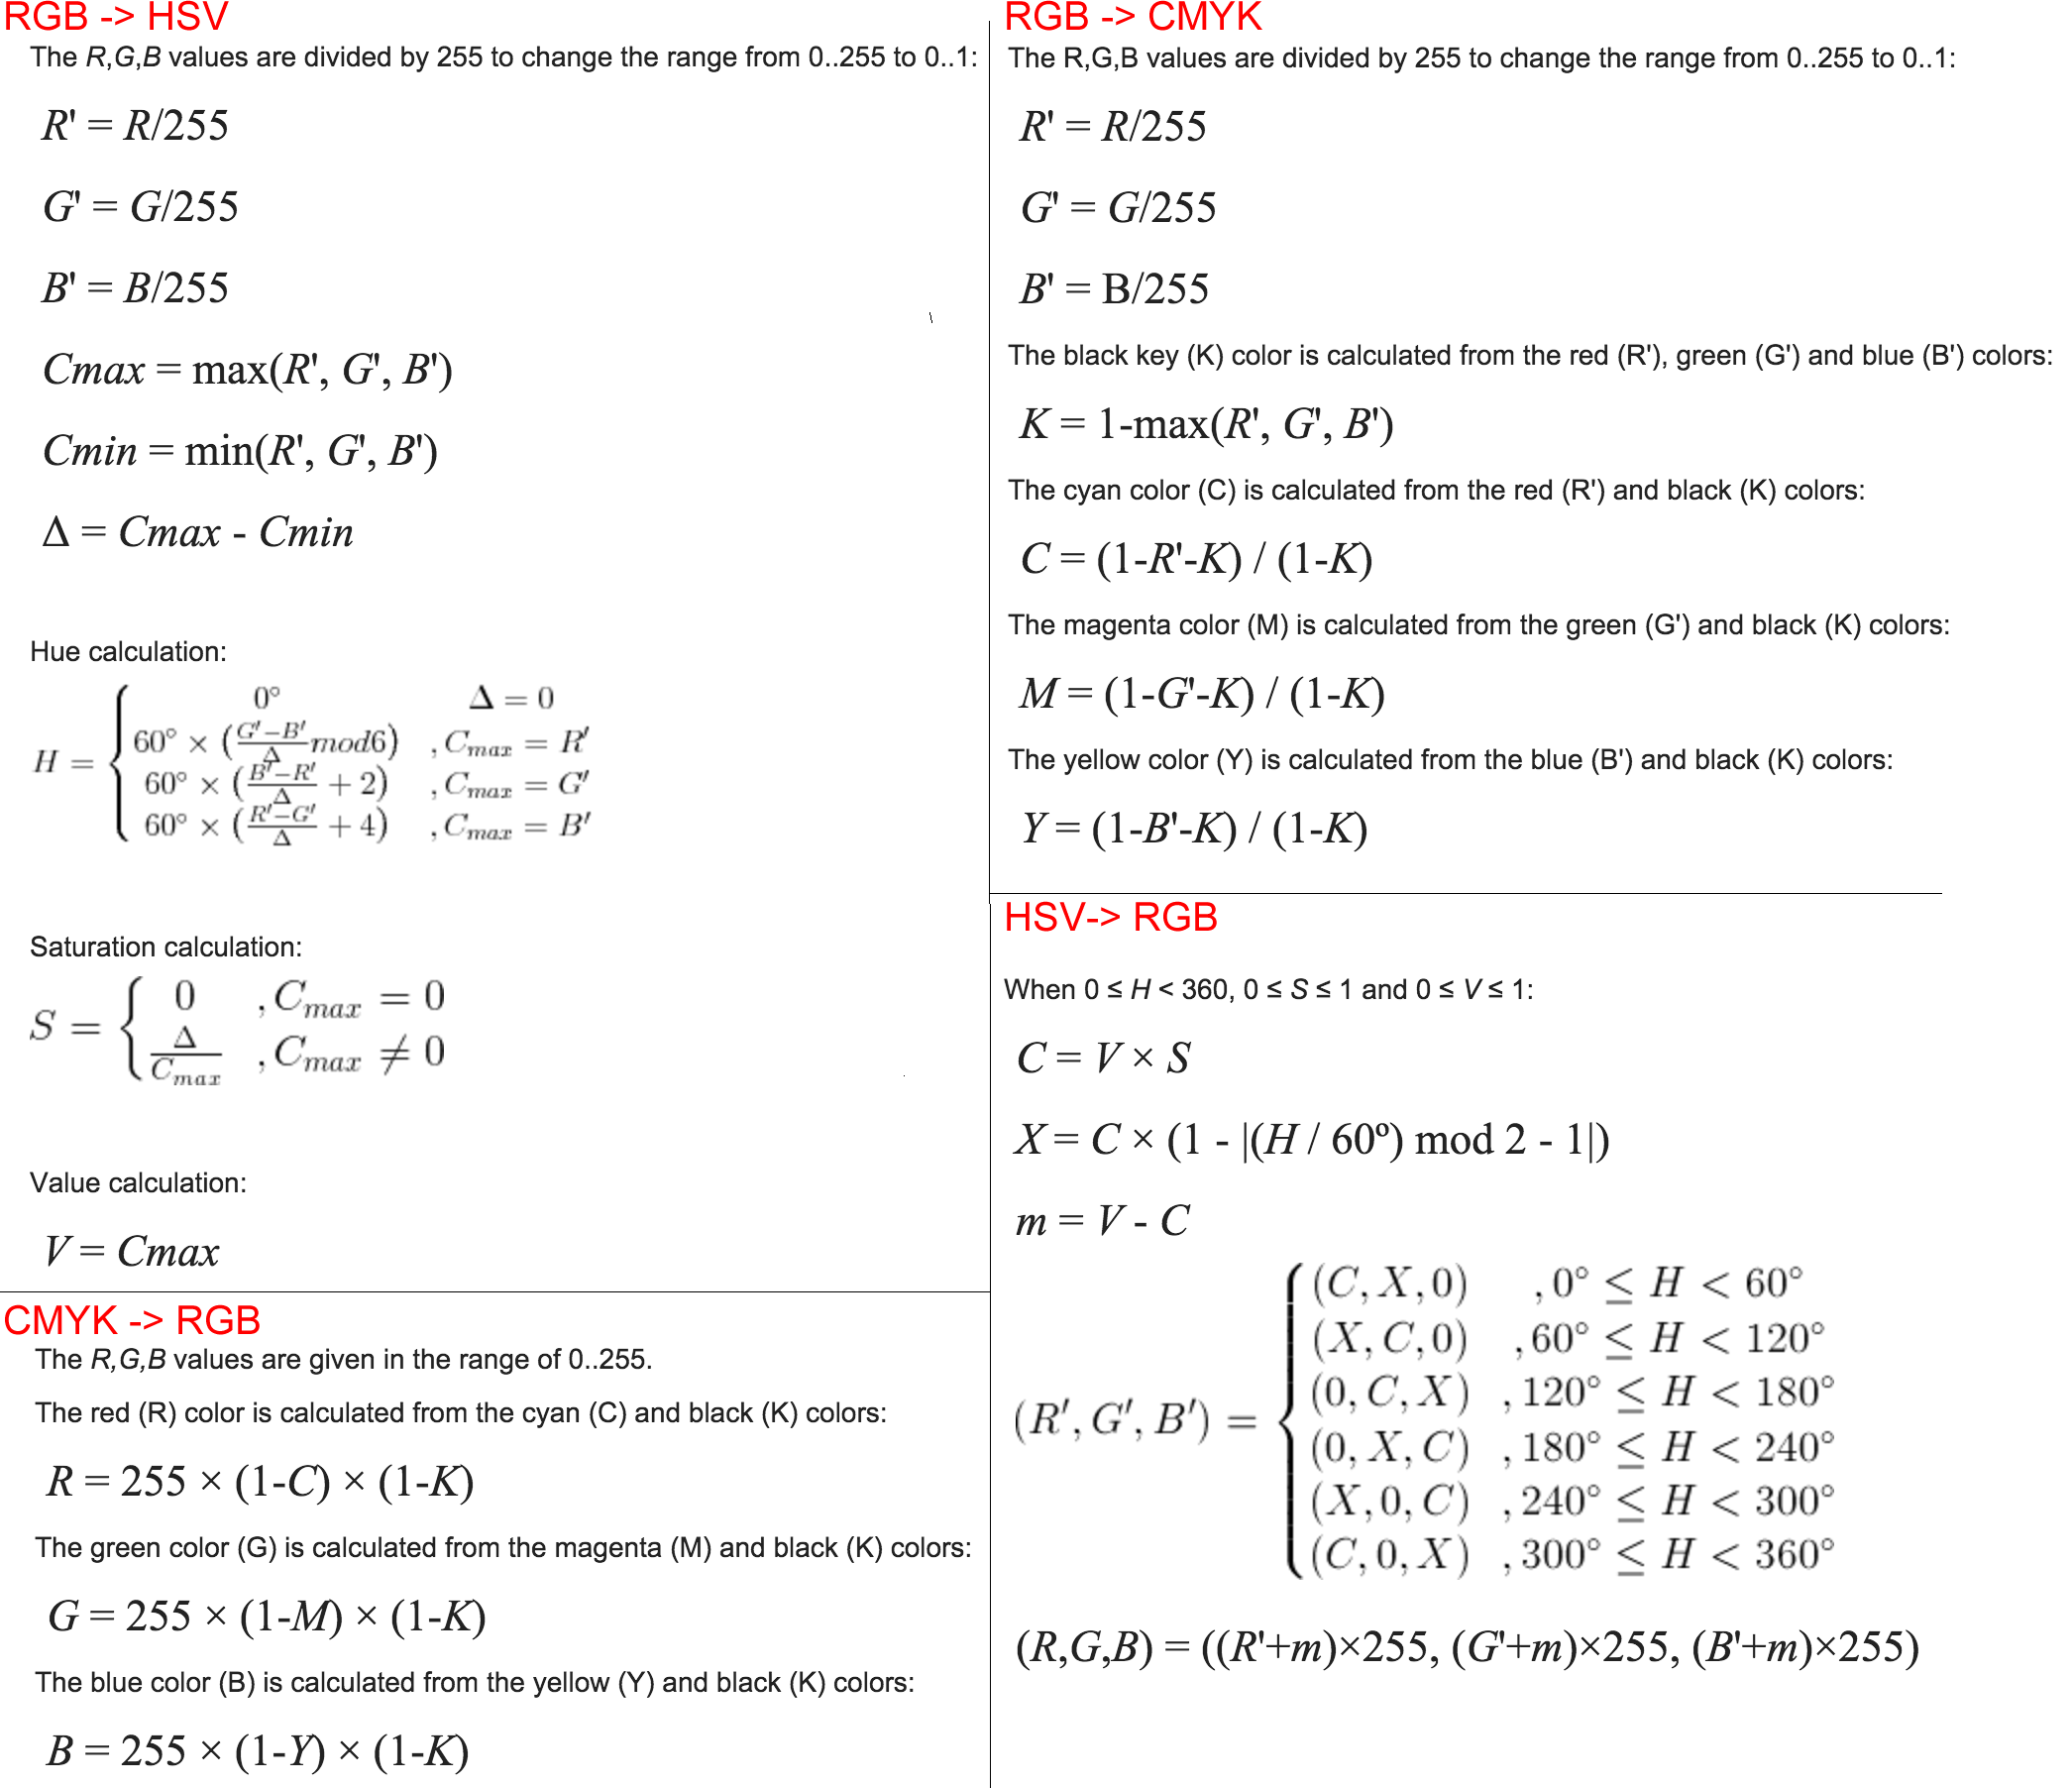
\includegraphics[width=1.0\linewidth]{fig/cheatsheet}
\end{figure}
\noindent

\subsection{Farbtabelle}
\begin{table}[!ht]
	\resizebox{\textwidth}{!}} & {\color[HTML]{FFFFFF} \textit{V \%}} & {\color[HTML]{FFFFFF} \textit{C}} & {\color[HTML]{FFFFFF} \textit{M}} & {\color[HTML]{FFFFFF} \textit{Y}} & {\color[HTML]{FFFFFF} \textit{C}} & {\color[HTML]{FFFFFF} \textit{M}} & {\color[HTML]{FFFFFF} \textit{Y}} & {\color[HTML]{FFFFFF} \textit{K}} \\ \hline
			\cellcolor[HTML]{000000}{\color[HTML]{000000} } & Schwarz & 0 & 0 & 0 & 0 & 0 & 0 & 1 & 1 & 1 & 0 & 0 & 0 & 1 \\ \hline
			& Weiss & 255 & 255 & 255 & 0 & 0 & 100 & 0 & 0 & 0 & 0 & 0 & 0 & 0 \\ \hline
			\cellcolor[HTML]{FF0000} & Rot & 255 & 0 & 0 &  & 100 & 100 & 0 & 1 & 1 & 0 & 1 & 1 & 0 \\ \hline
			\cellcolor[HTML]{00FF00} & Grün & 0 & 255 & 0 & 120 & 100 & 100 & 1 & 0 & 1 & 1 & 0 & 1 & 0 \\ \hline
			\cellcolor[HTML]{0000FF} & Blau & 0 & 0 & 255 & 240 & 100 & 100 & 1 & 1 & 0 & 1 & 1 & 0 & 0 \\ \hline
			\cellcolor[HTML]{FFFF00} & Yellow & 255 & 255 & 0 & 600 & 100 & 100 & 0 & 0 & 1 & 0 & 0 & 1 & 0 \\ \hline
			\cellcolor[HTML]{00FFFF} & Cyan & 0 & 255 & 255 & 180 & 100 & 100 & 1 & 0 & 0 & 1 & 0 & 0 & 0 \\ \hline
			\cellcolor[HTML]{FF00FF} & Magenta & 255 & 0 & 255 & 300 & 100 & 100 & 0 & 1 & 0 & 0 & 1 & 0 & 0 \\ \hline
			\cellcolor[HTML]{003200} & Dunkelgrün & 0 & 50 & 0 & 120 & 100 & 19.6 & 1 & 0.803921568627451 & 1 & 1 & 0 & 1 & 0.804 \\ \hline
			\cellcolor[HTML]{241409} & Braun & 36 & 20 & 9 & 24 & 75 & 14.1 & 0.8588235294117648 & 0.9215686274509804 & 0.9647058823529412 & 0 & 0.444 & 0.75 & 0.859 \\ \hline
			\cellcolor[HTML]{BEBEBE} & Grau & 190 & 190 & 190 & 0 & 0 & 74.5 &  &  &  & 0 & 0 & 0 & 0.255 \\ \hline
			\cellcolor[HTML]{FFA500} & Orange & 255 & 165 & 0 & 39 & 100 & 100 & 0 & 0.3529411764705882 & 1 & 0 & 0.353 & 1 & 0 \\ \hline
		\end{tabular}}
	\end{table}